%\documentclass{beamer}
\documentclass[mathserif,10pt]{beamer}

\usepackage{beamerthemesplit}
\usepackage{graphics}
\usepackage{epsfig}
\usepackage{algorithm}
\usepackage{verbatim}
\usepackage{listings}
\usepackage{framed}
\usepackage{pstricks}
\usepackage{pst-node,pst-tree}
\usepackage{pst-rel-points}
\usepackage{flexiprogram}
\usepackage[UKenglish]{babel}
\usepackage{hyperref}
\usepackage{pst-coil}
\usepackage{color}
\usepackage{epsfig}
\usepackage{tikz}
\usepackage{multirow}

\usefonttheme{serif}

\newcommand{\cmt}[1]{}
\newcommand{\epsilonset}{\ensuremath{\{\epsilon\}}}
\newcommand{\epsilonpairset}{\ensuremath{\{\epsilon,\epsilon\}}}
\newcommand{\num}[1]{\ensuremath{|#1|}}
\newcommand{\upath}{\ensuremath{\mathcal{U}}}
\newcommand{\mb}[1]{\mbox{{\tt #1}}}
\newcommand{\ttf}[1]{{\tt #1}}
\newcommand{\rtarrow}{$\rightarrow$}
\newcommand{\Tree}{{\tt Tree}}
\newcommand{\Dag}{{\tt Dag}}
\newcommand{\Cycle}{{\tt Cycle}}
\newcommand{\p}{\ensuremath{p}}
\newcommand{\q}{\ensuremath{q}}
\newcommand{\s}{\ensuremath{s}}
\newcommand{\myr}{\ensuremath{r}}
\newcommand{\shape}{\mbox{shape}}
\newcommand{\drct}{\ensuremath{D}}
\newcommand{\indrct}{\ensuremath{I}}
\newcommand{\heap}{\ensuremath{\mathcal{H}}}
\newcommand{\fields}{\ensuremath{\mathcal{F}}}
\newcommand{\DFM}[2]{\ensuremath{D_F[#1,#2]}}
\newcommand{\IFM}[2]{\ensuremath{I_F[#1,#2]}}
\newcommand{\nat}{\ensuremath{\mathcal{N}}}
\newcommand{\fieldD}[2]{\ensuremath{{#1}_{#2}^\drct}}
\newcommand{\fieldI}[3]{\ensuremath{{#1}_{#2}^{\indrct#3}}}
\newcommand{\subC}{\mbox{\scalebox{0.6}{\Cycle}}}
\newcommand{\subD}{\mbox{\scalebox{0.6}{\Dag}}}
\newcommand{\false}{\textbf{False}}
\newcommand{\true}{\textbf{True}}
%\noindent

\setcounter{tocdepth}{1}
\lstset{language=[ANSI]C}
\lstset{% general command to set parameter(s)
basicstyle=\footnotesize\tt, % print whole listing small
identifierstyle=, % nothing happens
commentstyle=\color{red}, % white comments
showstringspaces=false, % no special string spaces
lineskip=1pt,
captionpos=b,
frame=single,
breaklines=true
%\insertauthor[width={3cm},center,respectlinebreaks]
}
\lstset{classoffset=0,
morekeywords={},keywordstyle=\color{black},
classoffset=1,
classoffset=0}% restore default

%\usetheme{Warsaw}
\usetheme{CambridgeUS}
%\usetheme{Antibes}
%\usecolortheme{lily}
%\useinnertheme{rectangles} 
%\useoutertheme{infolines} 
%\setbeamercolor{alerted text}{fg=cyan}
%\beamertemplatetransparentcovereddynamicmedium
%\definecolor{bbrown}{rgb}{.6588,.4,.1647}
%\definecolor{blueviolet}{rgb}{.098039216,.050980392,.929411765}
%\definecolor{periwinkle}{rgb}{.423529412,.458823529,.988235294}
%\mode<presentation>
%{ \usetheme{boxes} }
\usecolortheme{dolphin}

\title{Precise Shape Analysis Using Field Sensitivity}
\author[Presented by: Sandeep Dasgupta]{\large{\textbf{Sandeep Dasgupta}}
\newline \small{Supervisors}
\newline \large{\textbf{Prof. Amey Karkare}}
\newline \small{\&}
\newline \large{\textbf{Prof. Sanjeev K. Aggarwal}}
}
\institute[CSE, IIT Kanpur]{\textbf{Department of Computer Science and Engineering}
\newline \textbf{Indian Institute of Technology, Kanpur}}
\date{June 24, 2011}
%\begin{comment}
\begin{document}

\begin{frame}
\titlepage
\end{frame}
\usebeamertemplate{mytheme}

\AtBeginSection[]
{
\begin{frame}<beamer>
\frametitle{Outline}
\tableofcontents[currentsection]
\end{frame}
}

\section{Introduction}
\subsection{Introduction}
\frame
{
	\frametitle{\subsecname}
	\uncover<1>{\textbf{Shape Analysis : } Class of techniques that statically approximate the
      run-time structures created on the heap.}
	\begin{figure}
  	\begin{center}
  
    \scalebox{.65}{
		\begin{tabular}[htbp]{ |c |  c |}
    	\hline
    	& \multirow{15}{*}{ 
			$\begin{array}{lcl}
		w.\shape == Tree &\Rightarrow& \mbox{ p.f$_2$.l.P and p.f$_2$..r.P$^{\prime}$ are disjoint. } \\ \\
		\q.\shape == Dag &\Rightarrow& \mbox{ p.f$_1$.f$_1$ and p.f$_1$.f$_2$.P are disjoint, where P } \\
		                 && \mbox{is a non-null path.} \\ \\
		\s.\shape == Cycle &\Rightarrow& \mbox{Disjoint-ness of paths  p.f$_3$.P and p.f$_3$.P$^{\prime}$} \\
							&& \mbox{ cannot be confirmed, where atleast one of} \\
							&& \mbox{P \& P$^{\prime}$ is non-null path.}
			\end{array}$
		} \\
      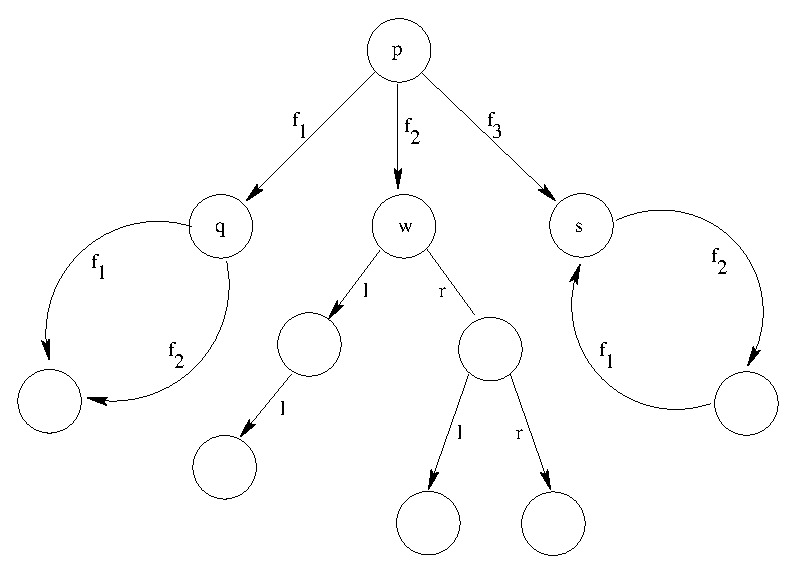
\includegraphics[scale=0.6]{Figure/figure_1}
      & \\
     (a) Heap structure & 
     (b) Some properties inferred from shape analysis. \\
     \hline
    \end{tabular}
	}
  	\end{center}
	\end{figure}
}

\subsection{Application}
\frame
{
	\frametitle{\subsecname}
		
	\begin{figure}
  	\begin{center}
  
    \scalebox{.80}{
		\begin{tabular}[htbp]{ | c | c  |}
    	\hline
    	& \multirow{3}{*}{ {\tt
\begin{program}{0}
%  \FL\ \ldots
  \UNL{0} void treeAdd(tree p) \{
  \UNL{1}  if(p == NULL)
  \UNL{2} return;
  \NL{1}     tl = p$\rightarrow$left;
  \NL{1}     \tikz[baseline]{\node[fill=blue!20,anchor=base](t1){treeAdd(tl);};}
  \NL{1}      tr = p$\rightarrow$right;
  \NL{1}     \tikz[baseline]{\node[fill=blue!20,anchor=base](t3){treeAdd(tr);};}
  \UNL{1}	p\rtarrow{num} = tl\rtarrow{num} + tr\rtarrow{num};
  \UNL{0} \}
\end{program}
}
} \\
      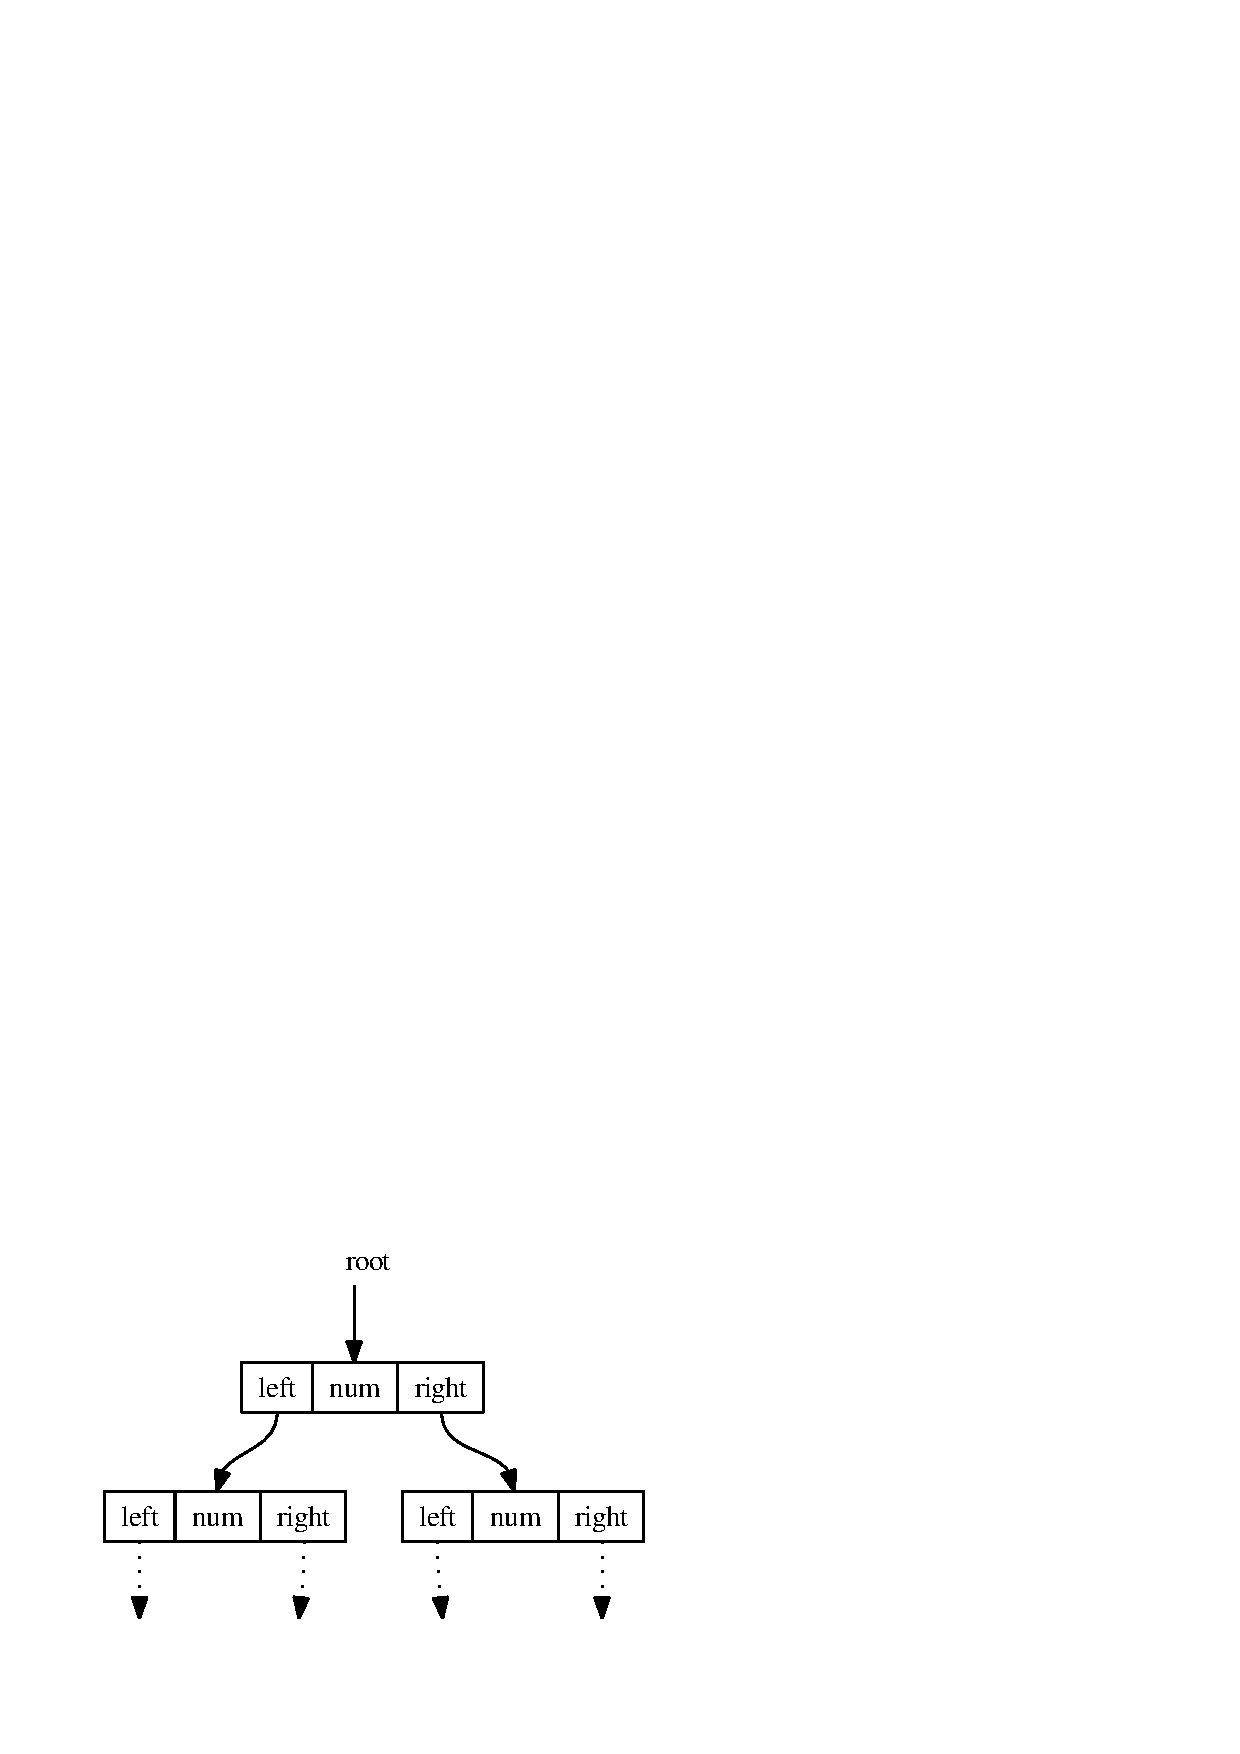
\includegraphics[scale=0.6]{tree_grph}
      & \\
     (a) Heap structure & 
     (b Function traversing the data structure. \\
     \hline
    \end{tabular}
	}
  	\end{center}
	\end{figure}

	\begin{center}
	(p.shape $==$ Tree) $\Rightarrow$ {\tt S2} and {\tt S4} can be executed in parallel.
  	\end{center}
}

\cmt{ NOT INCLUDED
\subsection{Programming Model}
\frame
{
	\frametitle{\subsecname}
	
\begin{figure}
  \begin{center}
  
    \scalebox{.8}{\begin{tabular}{ | c | c | c | c |}
   \hline
   & Before execution & Statement & After execution \\
   \hline
    Allocations & \begin{pspicture}(0,3)(2,4)
\psset{linecolor=blue}
\pscircle(1.3,3.5){.3}
\rput(0.2,3.5){\psframebox*{\scalebox{1}{\ttf{p}}}}
\end{pspicture}
 & \ttf{p = malloc()} & \begin{pspicture}(0,3)(2,4)
\psset{linecolor=blue}
\pscircle(1.3,3.5){.3}
\psset{linecolor=black}
\psline[linewidth=1pt,linearc=.5]{->}(0.3,3.5)(1,3.5)
\rput(0.2,3.5){\psframebox*{\scalebox{1}{\ttf{p}}}}
\end{pspicture}
\\
    \hline
    \multirow{3}{*}{Pointer Assignments} & \begin{pspicture}(0,3)(2,4)
\psset{linecolor=blue}
\pscircle(1.3,3.5){.3}
\psset{linecolor=black}
\psline[linewidth=1pt,linearc=.5]{->}(0.4,3.5)(1,3.5)
\rput(0.2,3.5){\psframebox*{\scalebox{1}{\ttf{q}}}}
\end{pspicture}
 & \ttf{p = q} & \begin{pspicture}(0,3.1)(2,4)
\psset{linecolor=blue}
\pscircle(1.3,3.5){.3}
\psset{linecolor=black}
\psline[linewidth=1pt,linearc=.5]{->}(0.3,3.8)(1,3.5)
\psline[linewidth=1pt,linearc=.5]{->}(0.3,3.2)(1,3.5)
\rput(0.2,3.8){\psframebox*{\scalebox{1}{\ttf{q}}}}
\rput(0.2,3.2){\psframebox*{\scalebox{1}{\ttf{p}}}}
\end{pspicture}
 \\
    \cline{2-4}
    & \begin{pspicture}(0,3)(3,4)
\psset{linecolor=blue}
\pscircle(1.3,3.5){.3}
\pscircle(2.7,3.5){.3}
\psset{linecolor=black}
\psline[linewidth=1pt,linearc=.5]{->}(0.4,3.5)(1,3.5)
%\psline[linewidth=1pt,linearc=.5,linecolor=red]{->}(1.6,3.5)(2.4,3.5)
\psline[linewidth=1pt,linearc=.5]{->}(1.6,3.5)(2.4,3.5)
\rput(0.2,3.5){\psframebox*{\scalebox{1}{\ttf{q}}}}
\rput(2,3.8){\psframebox*{\scalebox{1}{\ttf{f}}}}
\end{pspicture}
 & \ttf{p = q\rtarrow{f}} & \begin{pspicture}(0,3)(3,4.2)
\psset{linecolor=blue}
\pscircle(1.3,3.6){.3}
\pscircle(2.7,3.6){.3}
\psset{linecolor=black}
\psline[linewidth=1pt,linearc=.5]{->}(0.4,3.6)(1,3.6)
\psline[linewidth=1pt,linearc=.5]{->}(1.6,3.6)(2.4,3.6)
\psline[linewidth=1pt,linearc=.5]{->}(1.8,3.1)(2.4,3.6)
\rput(0.2,3.6){\psframebox*{\scalebox{1}{\ttf{q}}}}
\rput(2,3.9){\psframebox*{\scalebox{1}{\ttf{f}}}}
\rput(1.6,3.1){\psframebox*{\scalebox{1}{\ttf{p}}}}
\end{pspicture}
 \\
    \cline{2-4}
    & \begin{pspicture}(0,3)(2,4)
\psset{linecolor=blue}
\pscircle(1.3,3.5){.3}
\psset{linecolor=black}
\psline[linewidth=1pt,linearc=.5]{->}(0.3,3.5)(1,3.5)
\rput(0.2,3.5){\psframebox*{\scalebox{1}{\ttf{p}}}}
\end{pspicture}
 & \ttf{p = NULL} & \begin{pspicture}(0,3)(2,4)
\psset{linecolor=blue}
\pscircle(1.3,3.5){.3}
\rput(0.2,3.5){\psframebox*{\scalebox{1}{\ttf{p}}}}
\end{pspicture}
 \\
     \hline
     \multirow{2}{*}{Structure updates} & \begin{pspicture}(0,3)(3,4)
\psset{linecolor=blue}
\pscircle(1.3,3.5){.3}
\pscircle(2.7,3.5){.3}
\psset{linecolor=black}
\psline[linewidth=1pt,linearc=.5]{->}(0.4,3.5)(1,3.5)
\psline[linewidth=1pt,linearc=.5]{->}(1.6,3.5)(2.4,3.5)
\rput(0.2,3.5){\psframebox*{\scalebox{1}{\ttf{p}}}}
\rput(2,3.8){\psframebox*{\scalebox{1}{\ttf{f}}}}
\end{pspicture}
 & \ttf{p\rtarrow{f} = NULL} & \begin{pspicture}(0,3)(3,4.1)
\psset{linecolor=blue}
\pscircle(1.3,3.5){.3}
\pscircle(2.7,3.5){.3}
\psset{linecolor=black}
\psline[linewidth=1pt,linearc=.5]{->}(0.4,3.5)(1,3.5)
%\psline[linewidth=1pt,linearc=.5]{->}(1.6,3.5)(2.4,3.5)
\rput(0.2,3.5){\psframebox*{\scalebox{1}{\ttf{p}}}}
%\rput(2,3.8){\psframebox*{\scalebox{1}{\ttf{f}}}}
\end{pspicture}
 \\
     \cline{2-4}
     & \begin{pspicture}(0,3)(3,5.2)
\psset{linecolor=blue}
\pscircle(1.3,4.5){.3}
\pscircle(2.7,4.5){.3}
\pscircle(2,3.5){.3}
\psset{linecolor=black}
\psline[linewidth=1pt,linearc=.5]{->}(0.4,4.5)(1,4.5)
\psline[linewidth=1pt,linearc=.5]{->}(1.1,3.5)(1.7,3.5)
\psline[linewidth=1pt,linearc=.5]{->}(1.6,4.5)(2.4,4.5)
\rput(0.2,4.5){\psframebox*{\scalebox{1}{\ttf{p}}}}
\rput(2,4.8){\psframebox*{\scalebox{1}{\ttf{f}}}}
\rput(0.9,3.5){\psframebox*{\scalebox{1}{\ttf{q}}}}
\end{pspicture}
 & \ttf{p\rtarrow{f} = q} & \begin{pspicture}(0,3)(3,5.2)
\psset{linecolor=blue}
\pscircle(1.3,4.5){.3}
\pscircle(2.7,4.5){.3}
\pscircle(2,3.5){.3}
\psset{linecolor=black}
\psline[linewidth=1pt,linearc=.5]{->}(0.4,4.5)(1,4.5)
\psline[linewidth=1pt,linearc=.5]{->}(1.1,3.5)(1.7,3.5)
\psline[linewidth=1pt,linearc=.5]{->}(1.3,4.2)(2,3.8)
\rput(0.2,4.5){\psframebox*{\scalebox{1}{\ttf{p}}}}
\rput(1.6,4){\psframebox*{\scalebox{1}{\ttf{f}}}}
\rput(0.9,3.5){\psframebox*{\scalebox{1}{\ttf{q}}}}
\end{pspicture}
 \\
     \hline
    \end{tabular}}
  \end{center}
\end{figure}
}
}

\section{Related Work}
\subsection{Related Work}
\frame
{
	\frametitle{\subsecname}
	\begin{itemize}
	\item Work done by Ghiya et. al\footnote{Rakesh Ghiya and Laurie J. Hendren. Is it a Tree, a DAG, or a Cyclic graph? 
	a shape analysis for heap-directed pointers in C. In Proceedings of the 23rd ACM
	SIGPLAN-SIGACT symposium on Principles of programming languages, pages 1-15, January 1996.}
	
	\begin{itemize}
	\item Keeps interference and direction matrices between any two 
			pointer variables.
	\item Infer the shape of the structures as Tree, DAG or Cycle
	\item Conservatively identify the shapes.
	\end{itemize}
	\end{itemize}
}
\frame
{
	\frametitle{\subsecname}
	\begin{itemize}
	\item Work done by Sagiv et. al \footnote{Mooly Sagiv, Thomas Reps, and ReinhardWilhelm. Parametric shape analysis via
	3-valued logic. POPL 1999, pages 105-118, 1999.}
	
	\begin{itemize}
	\item Introduce the concepts of abstraction and re-materialization.
	\item Potentially exponential run-time in the number of predicates.
	\end{itemize}
	\end{itemize}
		
}
\cmt{
\frame
{
	\frametitle{\subsecname}
	\begin{itemize}
	\item Work done by Marron et. al \footnote{Mark Marron, Deepak Kapur, Darko Stefanovic, and Manuel Hermenegildo. A
static heap analysis for shape and connectivity: unified memory analysis: the base
framework. LCPC'06, pages 345-363, 2006.}
	
	\begin{itemize}
	\item Presents a data flow framework that uses heap graphs to model data flow values.
	\item The analysis uses technique similar to re-materialization, but the re-materialization is approximate and 
	may result in loss of precision.
	\end{itemize}
	\end{itemize}
		
}
}

\section{Motivation}
\subsection{Motivation}
\frame
{
	\frametitle{\subsecname}

	\cmt{For each pointer variable, our analysis computes the shape
attribute of the data structure pointed to by the variable.} 
We define the shape attribute $\p.\shape$
for a pointer $\p$ as follows:
%%
\begin{eqnarray*}
  \p.\shape = \left\{ \begin{array}{@{}rl@{}}
    \Cycle & \mbox{If a cycle can be reached from $\p$} \\ 
    \Dag & \mbox{Else if a DAG can be reached from $\p$} \\
    \Tree & \mbox{Otherwise} \\
  \end{array} \right.
\end{eqnarray*}
	\begin{center}
      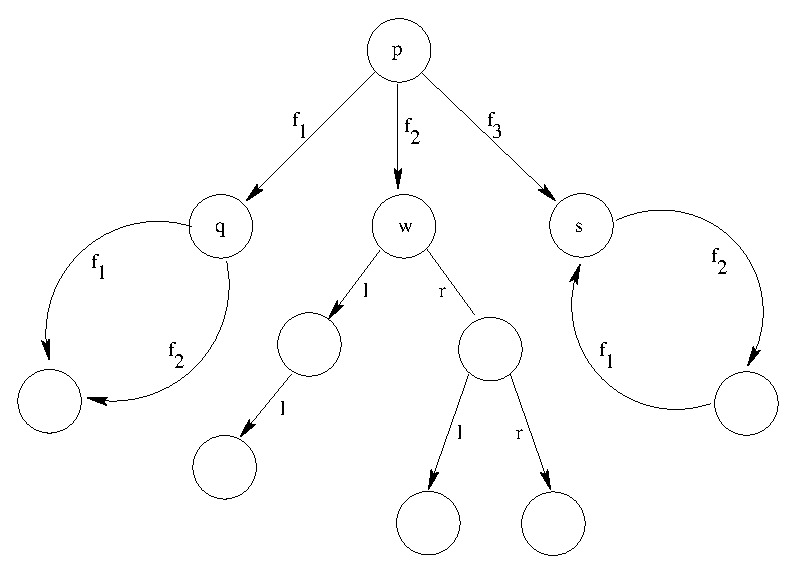
\includegraphics[scale=0.6]{Figure/figure_1}
	\end{center}
%%
\cmt{
where the heap is visualized as a directed graph, and cycle
and DAG have there natural graph-theoretic meanings.	}
}

\frame
{
	\frametitle{\subsecname}
	
\begin{figure}
  \begin{center}
  
    \scalebox{.8}{\begin{tabular}{ | l | c | c | c |c | c | }
   \hline
   \multirow{2}{*}{Statements} & \multirow{2}{*}{Heap Structure} & \multicolumn{2}{c|}{Actual Shape} &  \multicolumn{2}{c|}{Field Insensitive} \\
   \cline{3-6} 
   &  & p.shape & q.shape & p.shape & q.shape  \\
   \hline
	 &&&&& \\
    {\tt S1.} \ttf{p = malloc()} & \multirow{2}{*}{\begin{pspicture}(0,3)(3,4.2)
\psset{linecolor=blue}
\pscircle(.7,3.6){.3}
\pscircle(2.3,3.6){.3}
\rput(2.3,3.6){\psframebox*{\scalebox{.8}{\ttf{q}}}}
\rput(.7,3.6){\psframebox*{\scalebox{.8}{\ttf{p}}}}
\end{pspicture}
} &  \multirow{2}{*}{Tree} & \multirow{2}{*}{Tree} & \multirow{2}{*}{Tree} & \multirow{2}{*}{Tree} \\
    {\tt S2.} \ttf{q = malloc()} &  &  &&&\\
	 &&&&& \\
    \hline
	\pause
	 &&&&& \\
	{\tt S3.} \ttf{p$\rightarrow$f = q} &  \begin{pspicture}(0,3)(3,4.2)
\psset{linecolor=blue}
\pscircle(.7,3.6){.3}
\pscircle(2.3,3.6){.3}
\psset{linecolor=black}
\psline[linewidth=1pt,linearc=.5]{->}(1.0,3.6)(1.5, 3.9)(2.0,3.6)
\rput(2.3,3.6){\psframebox*{\scalebox{.8}{\ttf{q}}}}
\rput(1.5,4.1){\psframebox*{\scalebox{.8}{\ttf{f}}}}
\rput(.7,3.6){\psframebox*{\scalebox{.8}{\ttf{p}}}}
\end{pspicture}
 & Tree & Tree & Tree & Tree\\
	 &&&&& \\
     \hline
	\pause
	 &&&&& \\
	{\tt S4.} \ttf{p$\rightarrow$h = q} &  \begin{pspicture}(0,3)(3,4.2)
\psset{linecolor=blue}
\pscircle(.7,3.6){.3}
\pscircle(2.3,3.6){.3}
\psset{linecolor=black}
\psline[linewidth=1pt,linearc=.5]{->}(1.0,3.6)(1.5, 3.9)(2.0,3.6)
\psline[linewidth=1pt,linearc=.5]{->}(1.0,3.6)(1.5, 3.3)(2.0,3.6)
\rput(2.3,3.6){\psframebox*{\scalebox{.8}{\ttf{q}}}}
\rput(1.5,4.1){\psframebox*{\scalebox{.8}{\ttf{f}}}}
\rput(1.5,3.1){\psframebox*{\scalebox{.8}{\ttf{h}}}}
\rput(.7,3.6){\psframebox*{\scalebox{.8}{\ttf{p}}}}
\end{pspicture}
 & Dag & Tree & Dag & Tree \\
	 &&&&& \\
     \hline
    \end{tabular}}
  \end{center}
\end{figure}
}

\frame
{
	\frametitle{\subsecname}
	
\begin{figure}
  \begin{center}
  
    \scalebox{.8}{\begin{tabular}{ | l | c | c | c |c | c | }
   \hline
   \multirow{2}{*}{Statements} & \multirow{2}{*}{Heap Structure} & \multicolumn{2}{c|}{Actual Shape} &  \multicolumn{2}{c|}{Field Insensitive} \\
   \cline{3-6} 
   &  & p.shape & q.shape & p.shape & q.shape  \\
   \hline
	 &&&&& \\
	{\tt S5.} \ttf{q$\rightarrow$g = p} &  \begin{pspicture}(0,3)(3,4.2)
\psset{linecolor=blue}
\pscircle(.7,3.6){.3}
\pscircle(2.3,3.6){.3}

\psset{linecolor=black}
\psline[linewidth=1pt,linearc=.5]{->}(1.0,3.6)(1.5, 3.9)(2.0,3.6)
\psline[linewidth=1pt,linearc=.5]{->}(1.0,3.6)(1.5, 3.3)(2.0,3.6)
\psline[linewidth=1pt,linearc=.5]{->}(2.3,3.3)(1.5, 2.7)(0.7,3.3)

\rput(.7,3.6){\psframebox*{\scalebox{.8}{\ttf{p}}}}
\rput(2.3,3.6){\psframebox*{\scalebox{.8}{\ttf{q}}}}

\rput(1.5,4.1){\psframebox*{\scalebox{.8}{\ttf{f}}}}
\rput(1.5,3.1){\psframebox*{\scalebox{.8}{\ttf{h}}}}
\rput(1.5,2.5){\psframebox*{\scalebox{.8}{\ttf{g}}}}
\end{pspicture}
 & Cycle & Cycle & Cycle & Cycle\\
	 &&&&& \\
     \hline
	\pause
	 &&&&& \\
	{\tt S6.} \ttf{q$\rightarrow$g = null} &  \begin{pspicture}(0,3)(3,4.2)
\psset{linecolor=blue}
\pscircle(.7,3.6){.3}
\pscircle(2.3,3.6){.3}
\psset{linecolor=black}
\psline[linewidth=1pt,linearc=.5]{->}(1.0,3.6)(1.5, 3.9)(2.0,3.6)
\psline[linewidth=1pt,linearc=.5]{->}(1.0,3.6)(1.5, 3.3)(2.0,3.6)
\psset{linecolor=red}
\psline[linewidth=1pt,linearc=.5, linestyle=dashed]{->}(2.3,3.3)(1.5, 2.7)(0.7,3.3)

\rput(.7,3.6){\psframebox*{\scalebox{.8}{\ttf{p}}}}
\rput(2.3,3.6){\psframebox*{\scalebox{.8}{\ttf{q}}}}

\rput(1.5,4.1){\psframebox*{\scalebox{.8}{\ttf{f}}}}
\rput(1.5,3.1){\psframebox*{\scalebox{.8}{\ttf{h}}}}
\rput(1.5,2.5){\psframebox*{\scalebox{.8}{\ttf{g}}}}
\end{pspicture}
 & Dag & Tree & Cycle & Cycle \\
	 &&&&& \\
     \hline
	\pause
	 &&&&& \\
	{\tt S7.} \ttf{p$\rightarrow$h = null} &  \begin{pspicture}(0,3)(3,4.2)
\psset{linecolor=blue}
\pscircle(.7,3.6){.3}
\pscircle(2.3,3.6){.3}
\psset{linecolor=black}
\psline[linewidth=1pt,linearc=.5]{->}(1.0,3.6)(1.5, 3.9)(2.0,3.6)
\psset{linecolor=red}
\psline[linewidth=1pt,linearc=.5, linestyle=dashed]{->}(1.0,3.6)(1.5, 3.3)(2.0,3.6)
\psline[linewidth=1pt,linearc=.5, linestyle=dashed]{->}(2.3,3.3)(1.5, 2.7)(0.7,3.3)

\rput(.7,3.6){\psframebox*{\scalebox{.8}{\ttf{p}}}}
\rput(2.3,3.6){\psframebox*{\scalebox{.8}{\ttf{q}}}}

\rput(1.5,4.1){\psframebox*{\scalebox{.8}{\ttf{f}}}}
\rput(1.5,3.1){\psframebox*{\scalebox{.8}{\ttf{h}}}}
\rput(1.5,2.5){\psframebox*{\scalebox{.8}{\ttf{g}}}}
\end{pspicture}
 & Tree & Tree & Cycle & Cycle \\
	 &&&&& \\
     \hline
    \end{tabular}}
  \end{center}
\end{figure}
}

\frame
{
	\frametitle{\subsecname}
	
	Field insensitive shape analysis algorithms use conservative
	kill information. 
	\cmt{and hence they are, in general, unable to
	infer the shape transition from cycle to DAG or from DAG to
	Tree.}
	\begin{figure}
\centering
\scalebox{0.8}{
  \begin{tabular}{@{}cc@{}}
{\tt
      \begin{tabular}[b]{l}
        S1. p = malloc(); \\
        S2. q = malloc(); \\
        S3. p$\rightarrow$f = q; \\
        S4. p$\rightarrow$h = q; \\
        S5. q$\rightarrow$g = p; \\
        S6. q$\rightarrow$g = NULL;   \\
        S7. p$\rightarrow$h = NULL; 
      \end{tabular}
    }  &
    %\scalebox{0.80}{\begin{tabular}[b]{|c|@{}c@{}|@{}c@{}|}
    \begin{tabular}[b]{|c|@{}c@{}|@{}c@{}|}
      \hline
          {\bf After Stmt} & $D$ & $I$ \\ \hline
          {\tt S1}
          & \begin{tabular}{|c|cc|}
              {\tt } & $\p$  &  $\q$ \\ \hline
              $\p$ & 1  & 0 \\
              $\q$ & 0  & 0\\
			\hline
            \end{tabular} &
          \begin{tabular}{|c|cc|}
            {\tt } & $\p$  &  $\q$ \\ \hline
            $\p$ & 1  & 0 \\
            $\q$ & 0  & 0\\
			\hline
          \end{tabular}\\ \hline
         {\tt S2}
         & \begin{tabular}{|c|cc|}
             {\tt } & $\p$  &  $\q$ \\ \hline
             $\p$ & 1  & 0 \\
             $\q$ & 0  & 1\\
			\hline
           \end{tabular}&
		\begin{tabular}{|c|cc|}
		{\tt } & $\p$  &  $\q$ \\ \hline
		$\p$ & 1  & 0 \\
		$\q$ & 0  & 1\\
		\hline
		\end{tabular} \\ \hline
		{\tt S3}
	 & \begin{tabular}{|c|cc|} \hline 
	{\tt } & $\p$  &  $\q$ \\ \hline
	$\p$ & 1  & 1 \\
	$\q$ & 0  & 1\\
	\hline
	\end{tabular}&
	\begin{tabular}{|c|cc|} \hline 
	{\tt } & $\p$  &  $\q$ \\ \hline
	$\p$ & 1  & 1 \\
	$\q$ & 1  & 1\\
	\hline
	\end{tabular}\\ \hline
	{\tt S4}
	 & \begin{tabular}{|c|cc|} \hline 
	{\tt } & $\p$  &  $\q$ \\ \hline
	$\p$ & 1  & 1 \\
	$\q$ & 0  & 1\\
	\hline
	\end{tabular} &
	\begin{tabular}{|c|cc|} \hline 
	{\tt } & $\p$  &  $\q$ \\ \hline
	$\p$ & 1  & 1 \\
	$\q$ & 1  & 1\\
	\hline
	\end{tabular}\\ \hline
	{\tt S5, S6, S7}
	 & \begin{tabular}{|c|cc|} \hline 
	{\tt } & $\p$  &  $\q$ \\ \hline
	$\p$ & 1  & 1 \\
	$\q$ & 1  & 1\\
	\hline
	\end{tabular} &
	\begin{tabular}{|c|cc|} \hline 
	{\tt } & $\p$  &  $\q$ \\ \hline
	$\p$ & 1  & 1 \\
	$\q$ & 1  & 1\\
	\hline
	\end{tabular} \\ \hline
    \end{tabular} \\ 
     (a) A code fragment & 
     (b) \begin{tabular}[t]{@{}p{40mm}}
      Direction ($D$) and Interference ($I$) matrices as
      computed by Ghiya et. al.
    \end{tabular}
  \end{tabular}
	}
%\caption{A motivating example\label{fig:motivA}}
\end{figure}

}

\section{Our Analysis}
\subsection{Our Analysis}
\frame
{
	\frametitle{\subsecname}
	\begin{itemize}
	\item {\blue \textbf{Path Length Unbounded}}: \pause Approximate any path between two variables by the first field that is dereferenced on the path. 
	\pause
	\item  {\blue \textbf{Path Count Unbounded}}: \pause Use k-limiting to approximate the number of paths starting at a given field.
	\end{itemize}
}
\frame
{
	\frametitle{\subsecname}
	
	Our analysis remembers the path information using the following:
	\begin{itemize}
	\item  {\blue $D_F$}: Modified direction matrix. \cmt{ that stores the first fields of the paths between two pointers.}
	\pause
	\item {\blue $I_F$}: Modified interference matrix. \cmt{ that stores the pairs of first fields corresponding to the pairs of interfering paths.}
	\pause
	\item {\blue Boolean Variables}: For $f \in \fields, \p, \q \in \heap$, \\ 
			\begin{center}
			$f_{pq}$ == \true\ $ \Rightarrow$  $f$ field of $\p$ points directly to $\q$. 
			\end{center}
	
	\cmt{Field connectivity information: Remember the fields directly connecting two pointer variables.}
	\end{itemize}
}

\cmt{ NOT INCLUDED
\subsection{Notion of Path}
\frame
{
	\frametitle{\subsecname}
	\begin{itemize}
	\item A path from $\p$ to $\q$ is the sequence of pointer fields that need to be traversed in 
			the heap to reach from $\p$ to $\q$.
	\item Path length may be unbounded, so we consider only the first field of a path.
	\item For a path of length one (direct path) ($f_\drct$); For a path of length greater than one
			(indirect path) ($f_\indrct$).
	\item Possible to have multiple indirect paths starting with the same field : k-limiting, beyond k treat the number 
			of paths to be $\infty$.
	\end{itemize}
}
}

\frame
{
	\frametitle{\subsecname}
	\begin{figure}
\centering
\newcommand{\smf}{$f$}%%\scriptstyle f$}
\newcommand{\smh}{$h$}%%\scriptstyle h$}
\newcommand{\smg}{$g$}%%\scriptstyle g$}
\begin{tabular}{@{}cc@{}}
{\small \tt
    \begin{tabular}[b]{l}
      S1. q = p; \\
      S2. {\bf while}(...) \{ \\
      S3. \ \ \ \ q$\rightarrow$g = s; \\
      S4. \ \ \ \ q = q$\rightarrow$f; \\
      S5. \} \\
    \end{tabular}
  } &
 \scalebox{0.8}{ \psset{unit=1mm}
  \begin{pspicture}(0,0)(50,30)
    %%\psframe(0,0)(50,30)
    \putnode{q0}{origin}{3}{3}{}
    \putnode{q1}{q0}{0}{0}{\pscirclebox{\mbox{\p}}}
    \putnode{q2}{q1}{10}{0}{\pscirclebox[framesep=2.5]{\mbox{}}}
    \putnode{q3}{q2}{10}{0}{\mbox{\ldots}}
    \putnode{q4}{q3}{10}{0}{\pscirclebox{\mbox{\q}}}
    \putnode{q5}{q4}{10}{0}{\pscirclebox[framesep=2.5]{\mbox{}}}
    
    \ncline{->}{q1}{q2}
    \Bput[0.2]{\smf}
    \ncline{->}{q2}{q3}
    \Bput[0.2]{\smf}
    \ncline{->}{q3}{q4}
    \Bput[0.2]{\smf}
    \ncline{->}{q4}{q5}
    \Bput[0.2]{\smf}
    
    \putnode{s0}{q4}{15}{15}{\pscirclebox{\mbox{\s}}}
    \nccurve[angleA=90,angleB=145,ncurv=1]{->}{q1}{s0}
    \Aput[.1]{\smg}
    
    \putnode{t0}{q2}{0}{15}{\pscirclebox[framesep=2.5]{\mbox{}}}
    \nccurve[linestyle=dotted, dotsep=.5, angleA=-55,angleB=-165,
      ncurv=.2,nodesepA=-.3]{->}{t0}{s0}
    
    \ncline[linestyle=dotted, dotsep=.5]{->}{t0}{s0}
    \nccurve[linestyle=dotted, dotsep=.5,angleA=55,angleB=165,
      ncurv=.3,nodesepA=-.3]{->}{t0}{s0}
    

    \ncline[nodesepA=-.5,nodesepB=-.5]{->}{q1}{t0}
    \Aput[.1]{\smh}
    
    \ncline{->}{q2}{s0}
    \Bput[0.2]{\smg}
    \ncline[nodesepA=-.75,nodesepB=-.75]{->}{q4}{s0}
    \Bput[0.2]{\smg}
\end{pspicture}} \\
\scalebox{0.80}{ (a) A code fragment} & \scalebox{0.80}{ (b) 
  \begin{tabular}[t]{@{}p{95mm}}
    A possible heap graph for code in (a). Solid edges are the
    direct paths, dotted edges are the indirect paths.
  \end{tabular}}
  \end{tabular}
\caption{Paths in a heap graph}
\label{fig:pathsAndSets}
\end{figure}

	Assuming the limit $k \geq 3$, the path information between $\p$ and $\s$ can be represented by the set:
	$\{g^\drct, f^{\indrct\infty}, h^{\indrct 3} \}$. 
	If $k < 3$, then the set becomes: 
	$\{ g^\drct, f^{\indrct\infty}, h^{\indrct\infty} \}$
}

\cmt{ NOT INCLUDED
\subsection{Direction Matrix : $D_F$}
\frame
{
	\frametitle{\subsecname}
	\begin{definition}
\label{DFM_matrix}
Field sensitive Direction matrix
$D_F$ is a matrix that stores information 
about paths between two pointer variables.
Given $\p, \q \in
\heap, f \in \fields$:
\begin{eqnarray*}
  \epsilon & \in \DFM{p}{p}& \mbox{ where $\epsilon$
    denotes the empty path.} \\
  f^\drct  &\in  \DFM{p}{q} & \mbox{ if there is a direct
    path $f$ from $\p$ to $\q$.}\\
  f^{\indrct m} & \in  \DFM{p}{q} & 
  \mbox{\begin{tabular}[t]{p{70mm}}if there are $m$ indirect
      paths starting with field $f$ from $\p$ to $\q$ and $m
      \leq k.$
    \end{tabular}
  } \\
  f^{\indrct\infty} & \in  \DFM{p}{q} &
  \mbox{\begin{tabular}[t]{p{70mm}}if there are $m$ indirect
      paths starting with field $f$ from $\p$ to $\q$ and $m >
      k.$
  \end{tabular}}  
\end{eqnarray*}
\end{definition}
}

\subsection{Abstraction : $D_F$}
\frame
{
	\frametitle{\subsecname}
	Let \nat\ denote the set of natural numbers. We define the
following partial order for approximate paths used by our
analysis. For $ f \in \fields,\ m,n \in \nat,\ n \leq m$:
$$
\epsilon \sqsubseteq \epsilon, \quad 
f^\drct \sqsubseteq  f^\drct,  \quad
f^{\indrct\infty}  \sqsubseteq  f^{\indrct\infty}, \quad
f^{\indrct m} \sqsubseteq f^{\indrct\infty}, \quad
f^{\indrct n} \sqsubseteq f^{\indrct m} \enspace .
$$
The partial order is extended to set of paths $S_{P_1},
S_{P_2}$ as:
\begin{eqnarray*}
  S_{P_1} \sqsubseteq S_{P_2} &\Leftrightarrow& \forall \alpha \in
  S_{P_1}, \exists \beta \in S_{P_2}\ s.t. \alpha \sqsubseteq \beta \enspace .
\end{eqnarray*}
}

\subsection{Interference Matrix : $I_F$}
\frame
{
	\frametitle{\subsecname}
	\cmt{Two pointers $\p,\q \in \heap$ are said to
interfere if there exists $\s \in \heap$ such that both
$\p$ and $\q$ have paths reaching $\s$. Note that $\s$ could
be $\p$ (or $\q$) itself, in which case the path from $\p$
(from $\q$) is $\epsilon$.}

%FIELD SENSITIVE DIRECTION MATRIX 
\begin{definition}\label{IFM_matrix}
Field sensitive Interference matrix $I_F$ between
two pointers captures the ways in which these pointers are
interfering.  For $\p, \q, \s \in \heap, \p \not= \q$,
the following relation holds for $D_F$ and $I_F$: 
\begin{eqnarray*}
  \DFM{p}{s} \times \DFM{q}{s} &\sqsubseteq&
  \IFM{p}{q} \enspace . \label {eq:rel-df-if}
\end{eqnarray*}
\end{definition}
}

\subsection{Abstraction : $I_F$}
\frame
{
	\frametitle{\subsecname}
	For pair of paths:
\begin{eqnarray*}
  (\alpha, \beta) \sqsubseteq (\alpha', \beta') 
  \Leftrightarrow 
   (\alpha \sqsubseteq \alpha')  \wedge
  (\beta \sqsubseteq  \beta')
\end{eqnarray*}
For set of pairs of paths $R_{P_1}, R_{P_2}$:
\begin{eqnarray*}
  R_{P_1} \sqsubseteq R_{P_2} \Leftrightarrow \forall
  (\alpha, \beta) \in
  R_{P_1}, \exists (\alpha', \beta') \in
  R_{P_2}\ s.t. (\alpha, \beta) \sqsubseteq (\alpha', \beta')
\end{eqnarray*}
}
}

\subsection{Example : $D_F \mbox{ and } I_F$}
\frame
{
	\frametitle{\subsecname}
	\begin{figure}
\centering
\begin{tabular}{c@{$\qquad\qquad$}c}
\psset{unit=1.2mm}
\begin{pspicture}(0,0)(15,20)
	\psset{linecolor=black}
  \putnode{p0}{origin}{3}{9}{\pscirclebox{\p}}
  \putnode{q0}{p0}{5}{7}{\pscirclebox{\q}}
  %\putnode{r0}{p0}{0}{-14}{\pscirclebox{\myr}}
  \putnode{r0}{p0}{10}{0}{\pscirclebox{\myr}}
	\psset{linecolor=black}
  \ncline[nodesep=-.3]{<-}{p0}{q0}
  \aput[0.2](0.4){$\scriptstyle f$}
  \ncline{<-}{p0}{r0}
  \aput[0.2](0.4){$\scriptstyle g$}
%   %\ncline[nodesep=-.5]{->}{s0}{r0}
%   %\aput[0.2](0.2){$\scriptstyle f_5$}
%   \nccurve[angleA=45,angleB=0,linestyle=dotted,dotsep=0.2,ncurv=1,nodesepA=-.8]{->}{p0}{s0}
%   \aput[0.2](0.2){$\scriptstyle f_2$}
%   %\nccurve[angleA=180,angleB=225,linestyle=dotted,dotsep=0.2,ncurv=1,nodesepB=-.5]{->}{q0}{r0}
%   %\bput[0.2](0.2){$\scriptstyle f_4$}
\end{pspicture} &
\scalebox{0.8}{
\renewcommand{\arraystretch}{1.2}
\begin{tabular}[b]{|c|c|c|c|}
\hline
$D_F$          & \p                          & \q                             &  \myr  \\ \hline \hline 
\p 	           & $\{\epsilon\}$              & $\emptyset$            & $\emptyset$     \\ \hline 
\q             & $\{\fieldD{f}{}\}$                  & $\{\epsilon\}$                 & $\emptyset$   \\ \hline
\myr             & $\{\fieldD{g}{}\}$                 & $\emptyset$                    & $\{\epsilon\}$       \\ \hline
\end{tabular}} \\
\scalebox{0.80}{ (a) Heap graph} & \scalebox{0.80}{ (b) Direction Matrix}  \\ \\
% \multicolumn{2}{c}{
& \multirow{6}{*}{
\begin{tabular}{c}
$f_{\q\p} = \true$ \\
$f_{\p\q} = \false$ \\
$g_{\myr\p} = \true$ \\ 
\end{tabular}
} \\

\scalebox{0.80}{
\renewcommand{\arraystretch}{1.2}
\newcommand{\iwd}{0.23\columnwidth}
\begin{tabular}[b]{|c|c|c|c|}
\hline 
$\ I_F$     & $\p$	               & $\q$ &  $\myr$             \\ \hline \hline 
%%
$\p$ & $\{\epsilon, \epsilon\}$    & $\{(\epsilon, \fieldD{f}{}) \}$               & $\{(\epsilon, \fieldD{g}{})\}$      \\      \hline 
%%
$\q$       & $\{(\fieldD{f}{}, \epsilon)\}$                 & $\{\epsilon, \epsilon\}$          & $\{(\fieldD{f}{}, \fieldD{g}{})\}$         \\  \hline              
%%
$\myr$       & $\{(\fieldD{g}{}, \epsilon)\}$             & $\{(\fieldD{g}{}, \fieldD{f}{})\}$             & $\{\epsilon, \epsilon\}$         \\ \hline              
%%
\end{tabular}} &  \\
% } \\
% \multicolumn{2}{c}{\scalebox{0.80}{ (c) Interference Matrix} }
\scalebox{0.80}{(c) Interference Matrix}  & \scalebox{0.80}{(d) Bolean variables}
\end{tabular}
%\caption{A heap graph and its field sensitive path matrices\label{fig:DFM_IFM}}
\end{figure}

}	

\subsection{Boolean Functions}
\frame
{
	\frametitle{\subsecname}
	\begin{itemize}
	\item For each variable $\p \in \heap$, our analysis use attributes $\p_{\subD}$ and $\p_{\subC}$ to store boolean functions. \\
	\begin{center}
			$\p_{\subD} == \true \Rightarrow \p$ can reach a Dag  in the heap.\\
			$\p_{\subC} == \true \Rightarrow \p$ can reach a Cycle  in the heap. 
	\end{center}
	\pause
	\item The boolean functions consist of the values from:
		\begin{itemize}
			\item $D_F$
			\item $I_F$ 
			\item Boolean variables
		\end{itemize}	
	\pause
	\item An Example:
	$$
			\p_{\subC} = f_{\p\q} \wedge \num{D_F[\q,\p]} \geq 1
	$$		
	\end{itemize}
}

\frame
{
	\frametitle{\subsecname}
	\cmt{\begin{itemize}
	\item The shape of \p, \p.\shape, can be obtained by evaluating the functions for the attributes $\p_{\subC}$ and
          $\p_{\subD}$, and using following Table.}
		  \begin{table}
			\caption{Determining shape from boolean
			  attributes}
			\begin{center}
			%\begin{tabular*}{0.75\textwidth}{@{\extracolsep{\fill}} cccc|c }
			\begin{tabular}{|cc|cc|c| }
			\hline
			$\p_{\subC}$ &$\quad$ & $\p_{\subD}$ &$\quad$& $\p.\shape$ \\ 
			\hline
			\true  && Don't Care  && Cycle        \\ 
			\false  && \true          && DAG    \\ 
			\false  && \false          && Tree   \\ 
			\hline
			\end{tabular}
			\end{center}
		\end{table}

	\cmt{\end{itemize}}
}

\subsection{Analysis Framework}
\frame
{
	\frametitle{\subsecname}
	
	\begin{itemize}
	\item Forward data flow analysis framework. \cmt{ where the data flow values are the $D_F$, $I_F$ and 
	the boolean variables.}
	\pause
	\item On demand evaluation of boolean functions.
	\cmt{We do not evaluate the boolean functions immediately, but associate
the unevaluated functions with the statements. When we want to find out the shape at a given
statement, only then we evaluate the function using the $D_F$ and $I_F$ matrices, and the values of
boolean variables at that statement.}
	\cmt{\pause
	\item Field connectivity information is updated directly by the statement.}
	\end{itemize}
}

\subsection{Motivational Example Revisited}
\frame
{
	\frametitle{\subsecname}
	
\begin{figure}
  \begin{center}
  
    \scalebox{.80}{\begin{tabular}{ |@{}l@{ }|@{}c@{}|@{}c@{}|@{}c@{}|@{}c@{}|  }
   \hline
   \multirow{2}{*}{Statements} & \multirow{2}{*}{Heap Structure} & \multirow{2}{*}{Boolean Functions} &  \multicolumn{2}{@{}c@{}|}{Shape Inference}  \\
   \cline{4-5} 
   &  &  &   p.shape & q.shape  \\
   \hline
	 &&&& \\
    {\tt S1.} \ttf{p = malloc()} & \multirow{2}{*}{\begin{pspicture}(0,3)(3,4.2)
\psset{linecolor=blue}
\pscircle(.7,3.6){.3}
\pscircle(2.3,3.6){.3}
\rput(2.3,3.6){\psframebox*{\scalebox{.8}{\ttf{q}}}}
\rput(.7,3.6){\psframebox*{\scalebox{.8}{\ttf{p}}}}
\end{pspicture}
} &  
																				$\begin{array}{@{}c@{}}
																					p_{\subC} = \false  \qquad q_{\subC} = \false \\ 
																					p_{\subD} = \false  \qquad q_{\subD} = \false 
																				\end{array}$
																				& \multirow{2}{*}{Tree} & \multirow{2}{*}{Tree} \\
    {\tt S2.} \ttf{q = malloc()} &    &&&\\
	 &&&& \\
    \hline
	\pause
	 &&&& \\
	{\tt S3.} \ttf{p$\rightarrow$f = q} &  \begin{pspicture}(0,3)(3,4.2)
\psset{linecolor=blue}
\pscircle(.7,3.6){.3}
\pscircle(2.3,3.6){.3}
\psset{linecolor=black}
\psline[linewidth=1pt,linearc=.5]{->}(1.0,3.6)(1.5, 3.9)(2.0,3.6)
\rput(2.3,3.6){\psframebox*{\scalebox{.8}{\ttf{q}}}}
\rput(1.5,4.1){\psframebox*{\scalebox{.8}{\ttf{f}}}}
\rput(.7,3.6){\psframebox*{\scalebox{.8}{\ttf{p}}}}
\end{pspicture}
 & 
																				$\begin{array}{@{}c@{}}
																					p_{\subC} = (f_{\p\q} \wedge \num{D_F[q,p]} \geq 1) \\ \\
																					q_{\subC} = f_{\p\q} \wedge \num{D_F[q,p]} \geq 1 \\ \\
																					p_{\subD} = f_{\p\q} \wedge \num{I_F[\p,\q]} > 1 \\ \\
																					f_{\p\q} = \true
																				\end{array}$
																	  & Tree & Tree\\
	 &&&& \\
     \hline
	\pause
	 &&&& \\
	{\tt S4.} \ttf{p$\rightarrow$h = q} &  \begin{pspicture}(0,3)(3,4.2)
\psset{linecolor=blue}
\pscircle(.7,3.6){.3}
\pscircle(2.3,3.6){.3}
\psset{linecolor=black}
\psline[linewidth=1pt,linearc=.5]{->}(1.0,3.6)(1.5, 3.9)(2.0,3.6)
\psline[linewidth=1pt,linearc=.5]{->}(1.0,3.6)(1.5, 3.3)(2.0,3.6)
\rput(2.3,3.6){\psframebox*{\scalebox{.8}{\ttf{q}}}}
\rput(1.5,4.1){\psframebox*{\scalebox{.8}{\ttf{f}}}}
\rput(1.5,3.1){\psframebox*{\scalebox{.8}{\ttf{h}}}}
\rput(.7,3.6){\psframebox*{\scalebox{.8}{\ttf{p}}}}
\end{pspicture}
 & 
																				$\begin{array}{@{}c@{}}
																					\p_{\subD} = (f_{\p\q} \wedge \num{I_F[\p,\q]} > 1) \vee (h_{\p\q} \wedge \num{I_F[\p,\q]} > 1) \\ \\
																					f_{\p\q} = \true \qquad h_{\p\q} = \true
																				\end{array}$
																	  & Dag & Tree\\
	 &&&& \\
     \hline
    \end{tabular}}
  \end{center}
\end{figure}
}
\frame
{
	\frametitle{\subsecname}
	
\begin{figure}
  \begin{center}
  
    \scalebox{.80}{\begin{tabular}{ |@{}l@{ }|@{}c@{}|@{}c@{}|@{}c@{}|@{}c@{}|  }
   \hline
   \multirow{2}{*}{Statements} & \multirow{2}{*}{Heap Structure} & \multirow{2}{*}{Boolean Functions} &  \multicolumn{2}{@{}c@{}|}{Shape Inference}  \\
   \cline{4-5} 
   &  &  &   p.shape & q.shape  \\
     \hline
	 &&&& \\
	{\tt S5.} \ttf{q$\rightarrow$g = p} &  \begin{pspicture}(0,3)(3,4.2)
\psset{linecolor=blue}
\pscircle(.7,3.6){.3}
\pscircle(2.3,3.6){.3}

\psset{linecolor=black}
\psline[linewidth=1pt,linearc=.5]{->}(1.0,3.6)(1.5, 3.9)(2.0,3.6)
\psline[linewidth=1pt,linearc=.5]{->}(1.0,3.6)(1.5, 3.3)(2.0,3.6)
\psline[linewidth=1pt,linearc=.5]{->}(2.3,3.3)(1.5, 2.7)(0.7,3.3)

\rput(.7,3.6){\psframebox*{\scalebox{.8}{\ttf{p}}}}
\rput(2.3,3.6){\psframebox*{\scalebox{.8}{\ttf{q}}}}

\rput(1.5,4.1){\psframebox*{\scalebox{.8}{\ttf{f}}}}
\rput(1.5,3.1){\psframebox*{\scalebox{.8}{\ttf{h}}}}
\rput(1.5,2.5){\psframebox*{\scalebox{.8}{\ttf{g}}}}
\end{pspicture}
 	& 
																				$\begin{array}{@{}c@{}}
																					\p_{\subC} = (g_{\q\p} \wedge \num{D_F[\p,\q]} \geq 1) \\ \\
																					\p_{\subD} = (f_{\p\q} \wedge \num{I_F[\p,\q]} > 1) \vee (h_{\p\q} \wedge \num{I_F[\p,\q]} > 1) \\ \\
																					f_{\p\q} = \true \qquad h_{\p\q} = \true \qquad g_{\q\p} = \true 
																				\end{array}$
	
																		& Cycle & Cycle\\
	 &&&& \\
     \hline
	 \pause
	 &&&& \\
	{\tt S6.} \ttf{q$\rightarrow$g = null} &  \begin{pspicture}(0,3)(3,4.2)
\psset{linecolor=blue}
\pscircle(.7,3.6){.3}
\pscircle(2.3,3.6){.3}
\psset{linecolor=black}
\psline[linewidth=1pt,linearc=.5]{->}(1.0,3.6)(1.5, 3.9)(2.0,3.6)
\psline[linewidth=1pt,linearc=.5]{->}(1.0,3.6)(1.5, 3.3)(2.0,3.6)
\psset{linecolor=red}
\psline[linewidth=1pt,linearc=.5, linestyle=dashed]{->}(2.3,3.3)(1.5, 2.7)(0.7,3.3)

\rput(.7,3.6){\psframebox*{\scalebox{.8}{\ttf{p}}}}
\rput(2.3,3.6){\psframebox*{\scalebox{.8}{\ttf{q}}}}

\rput(1.5,4.1){\psframebox*{\scalebox{.8}{\ttf{f}}}}
\rput(1.5,3.1){\psframebox*{\scalebox{.8}{\ttf{h}}}}
\rput(1.5,2.5){\psframebox*{\scalebox{.8}{\ttf{g}}}}
\end{pspicture}
 	& 
																				$\begin{array}{@{}c@{}}
																					\p_{\subC} = (g_{\q\p} \wedge \num{D_F[\p,\q]} \geq 1) \\ \\
																					\p_{\subD} = (f_{\p\q} \wedge \num{I_F[\p,\q]} > 1) \vee (h_{\p\q} \wedge \num{I_F[\p,\q]} > 1) \\ \\
																					f_{\p\q} = \true \qquad h_{\p\q} = \true \qquad g_{\q\p} = \false 
																				\end{array}$
	
																		& Dag & Tree\\
	 &&&& \\
     \hline
	 \pause
	 &&&& \\
	{\tt S7.} \ttf{p$\rightarrow$h = null} &  \begin{pspicture}(0,3)(3,4.2)
\psset{linecolor=blue}
\pscircle(.7,3.6){.3}
\pscircle(2.3,3.6){.3}
\psset{linecolor=black}
\psline[linewidth=1pt,linearc=.5]{->}(1.0,3.6)(1.5, 3.9)(2.0,3.6)
\psset{linecolor=red}
\psline[linewidth=1pt,linearc=.5, linestyle=dashed]{->}(1.0,3.6)(1.5, 3.3)(2.0,3.6)
\psline[linewidth=1pt,linearc=.5, linestyle=dashed]{->}(2.3,3.3)(1.5, 2.7)(0.7,3.3)

\rput(.7,3.6){\psframebox*{\scalebox{.8}{\ttf{p}}}}
\rput(2.3,3.6){\psframebox*{\scalebox{.8}{\ttf{q}}}}

\rput(1.5,4.1){\psframebox*{\scalebox{.8}{\ttf{f}}}}
\rput(1.5,3.1){\psframebox*{\scalebox{.8}{\ttf{h}}}}
\rput(1.5,2.5){\psframebox*{\scalebox{.8}{\ttf{g}}}}
\end{pspicture}
 	& 
																				$\begin{array}{@{}c@{}}
																					\p_{\subC} = (g_{\q\p} \wedge \num{D_F[\p,\q]} \geq 1) \\ \\
																					\p_{\subD} = (f_{\p\q} \wedge \num{I_F[\p,\q]} > 1) \vee (h_{\p\q} \wedge \num{I_F[\p,\q]} > 1) \\ \\
																					f_{\p\q} = \true \qquad h_{\p\q} = \false \qquad g_{\q\p} = \false 
																				\end{array}$
	
																		& Tree & Tree\\
	 &&&& \\
     \hline
    \end{tabular}}
  \end{center}
\end{figure}
}

\section{Properties}
\subsection{Need for Boolean Variables}
\frame
{
	\frametitle{\subsecname}

	\begin{figure}[t]
  \centering
  \begin{tabular}{@{}lcc@{}}
    \scalebox{0.80}{
      \tt
      \begin{tabular}[b]{l}
        \qquad \qquad \ldots \\
        S1. r = s$\rightarrow$g;\\
        S2. p$\rightarrow$f = q;  \\
        S3. p$\rightarrow$f = NULL; \\
        \qquad \qquad \ldots \\
      \end{tabular}
    } &
    \scalebox{0.8}{\psset{unit=1mm}
    \begin{pspicture} (0,0)(30,16)
      \putnode{p0}{origin}{3}{3}{\pscirclebox[framesep=3pt]{\p}}
      \putnode{s0}{p0}{0}{10}{\pscirclebox[framesep=4pt]{\s}}
      \putnode{t0}{s0}{15}{0}{\pscirclebox[framesep=5pt]{\ }}
      \putnode{q0}{p0}{15}{0}{\pscirclebox[framesep=3pt]{\q}}
      \putnode{u0}{q0}{10}{5}{\pscirclebox[framesep=5pt]{\ }}

      \ncline{->}{s0}{t0}
      \Aput[0.1]{$g$}
      \ncline[nodesep=-0.5]{->}{t0}{p0}
      \Aput[0.1]{$f$}
      \ncline[nodesep=-0.5]{->}{t0}{u0}
      \Aput[0.1]{$g$}
      \ncline[nodesep=-0.5]{->}{q0}{u0}
      \Aput[0.1]{$h$}

    \end{pspicture}}
    &
    \scalebox{0.80}{
    \begin{tabular}[b]{|c|c|c|c|}
      \hline
	  {After} & $f_{pq}$ & $\IFM{r}{q}$                             	    & $\DFM{r}{p}$ \\ \hline
	  {\tt S1}       &  {\tt false}  &  $\upath \times \{h\}$                   & \upath \\ \hline
	  {\tt S2}       &  {\tt true}   &  $\upath \times \{h, \epsilon\}$  & \upath \\ \hline
	  {\tt S3}       &  {\tt false}  &  $\upath \times \{h, \epsilon\}$  & \upath \\ \hline
    \end{tabular}}  \\
    \scalebox{0.80}{(a) A code fragment} &
    \scalebox{0.80}{(b) \begin{tabular}[t]{p{37mm}}
    Heap Structure before {\tt S1} 
    \end{tabular}}
    &     
    \scalebox{0.80}{(c) \begin{tabular}[t]{p{43mm}}
        Values for boolean variable, $D_F$, and
        $I_F$ for relevant pointer fields.
    \end{tabular}}
      \\
  \end{tabular}
  \caption{Using boolean variables to improve
    precision \label{fig:conclusion}} 
\end{figure}

	\[ \upath \quad=\quad \epsilonset \cup \bigcup_{f\in\fields} \{f^{\drct},
f^{\indrct\infty}\} \]
	After {\tt S2},
	\begin{eqnarray*}
   \mb{r}_{\subD} = (f_{pq} \wedge (|\IFM{r}{q}| > 1))
   	&\qquad& f_{pq} = \true
 	\end{eqnarray*}
}

\subsection{Storage Requirement}
\frame
{
	\frametitle{\subsecname}
	\begin{eqnarray*}
\mbox{Space requirement for } D_F &:&  O(n^{2}* m) \\
\mbox{Space requirement for } I_F &:& O(n^{2} * m^2) \\
\mbox{Height and width of the expression tree} &:& \mbox{Polynomial in number} \\
												&& \mbox{of pointer instructions} \\
												&& \mbox{executed}
\end{eqnarray*}
}

\section{Test Results}
\subsection{Inserting an internal node in a singly linked list.}
\frame
{
	\frametitle{\subsecname}

	\newcommand{\on}{p} 
	\newcommand{\nn}{r}

\begin{figure}
\centering
\scalebox{0.80}{
\begin{tabular}{@{}ll@{}}
  {\small\tt
    \begin{tabular}[b]{l}
      S1. \on$\rightarrow$f = q; \\
      S2. \nn = malloc(); \\
      S3. \nn$\rightarrow$f = q;  \\
      S4. \on$\rightarrow$f = \nn;  
    \end{tabular}
  } &
  \scalebox{0.80}{
    \begin{tabular}[b]{|c||c|c|c|}
      \hline
          {\bf After} & Actual Shape & Field Insensitive
          Analysis & Field Sensitive Analysis \\ 
          \hline \hline
	  {\tt S1}       & Tree		  & Tree    & Tree \\ \hline
	  {\tt S2}       & Tree		  & Tree    & Tree \\ \hline
	  {\tt S3}       & Tree		  & Tree    & Tree \\ \hline
	  {\tt S4}       & Tree		  & DAG(at {\tt \on})    & Tree \\ \hline
    \end{tabular}
  } \\
  \multicolumn{2}{c}{\scalebox{1.00}{(a) Insertion of an
      internal node in a singly linked list }}
	  \end{tabular}}
	  \end{figure}
	  Boolean function generated after {\tt S4}:
\begin{eqnarray*}
  \p_{\subD} &=&   (f_{\p\q} \wedge (\num{I_F[\p\q]} > 1)) 
  \vee  (f_{\p\myr} \wedge (\num{I_F[\p\myr]} > 1)), \\
  f_{\p\myr} &=& \true, \qquad\qquad  f_{\p\q} = \false \enspace. 
\end{eqnarray*}
}
\subsection{Recursively Swapping Binary Tree.}
\frame
{
	\frametitle{\subsecname}

	\newcommand{\on}{p} 
	\newcommand{\nn}{r}

\begin{figure}
\centering
\scalebox{0.80}{
\begin{tabular}{@{}ll@{}}
{\small \tt
    \begin{tabular}[b]{l}
      mirror(tree T) \{ \\
      S1.    L  = T->left; \\
      S2.    R = T->right; \\
      S3.    mirror(L); \\
      S4.    mirror(R); \\
      S5.    T->left = R; \\
      S6.    T->right = L; \\
      \}  
    \end{tabular}
  } &
  \scalebox{0.80}{
    \begin{tabular}[b]{|c||c|c|c|}
      \hline
          {\bf After} & Actual Shape & Field Insensitive
          Analysis & Field Sensitive Analysis \\ 
          \hline \hline
	  {\tt S1}       & Tree		  & Tree    & Tree \\ \hline
	  {\tt S2}       & Tree		  & Tree    & Tree \\ \hline
	  {\tt S5}       & Dag (at T)	  & Dag (at T)    & Dag (at T) \\ \hline
	  {\tt S6}       & Tree		  & Dag (at T)    & Tree \\ \hline
    \end{tabular}
  } \\
  \multicolumn{2}{c}{\scalebox{1.00}{(c) Computing mirror
      image of a  binary tree.}}
\end{tabular}}
\end{figure}

Boolean functions generated after {\tt S5}:
\begin{eqnarray*}
  T_{\subD} &=&   (left_{T,R} \wedge \num{I_F[T,R]} > 1) \\ 
  left_{T,R} &=& \true 
\end{eqnarray*}
}

\section{Future Work}
\subsection{Future Work}
\frame
{
	\frametitle{\subsecname}
	\begin{itemize}
	\item We use a very simple inter procedural framework to handle
function calls, that computes safe approximate summaries to
reach fix point .  Our next challenge is to develop a better
inter procedural analysis to handle function calls more
precisely. 
	\item To extend our shape analysis
technique to handle more of frequently occurring programming
patterns.
     \item To develop a prototype model using
GCC framework to show the effectiveness on large
benchmarks. 
	\end{itemize}
}

\begin{frame}[plain]

	\begin{center}
	\Huge{\emph{\blue Thank You }}
	\end{center}
\end{frame}
\end{document}

